% Generated by scripts/analysis/render_poster_matrices.py (adaptive).
% source_csv=/Users/rasikaramanan/Documents/usc/by_semester/f26/csci566/project/synthea-prep/experiments/results_all_variants/experiment_results.csv
% source_csv_sha256=bffb8776b7c15ecdee40e8de6b8b80c726e05d5be065b54a309b8e8bc9d9b5c2
\documentclass[border=2pt]{standalone}
\usepackage[T1]{fontenc}
\usepackage[scaled=0.95]{helvet}
\renewcommand{\familydefault}{\sfdefault}
\usepackage{tikz}
\ifdefined\pdfinfoomitdate\pdfinfoomitdate=1\fi
\ifdefined\pdftrailerid\pdftrailerid{}\fi
\setlength{\parindent}{0pt}
\begin{document}
\begin{minipage}{16cm}
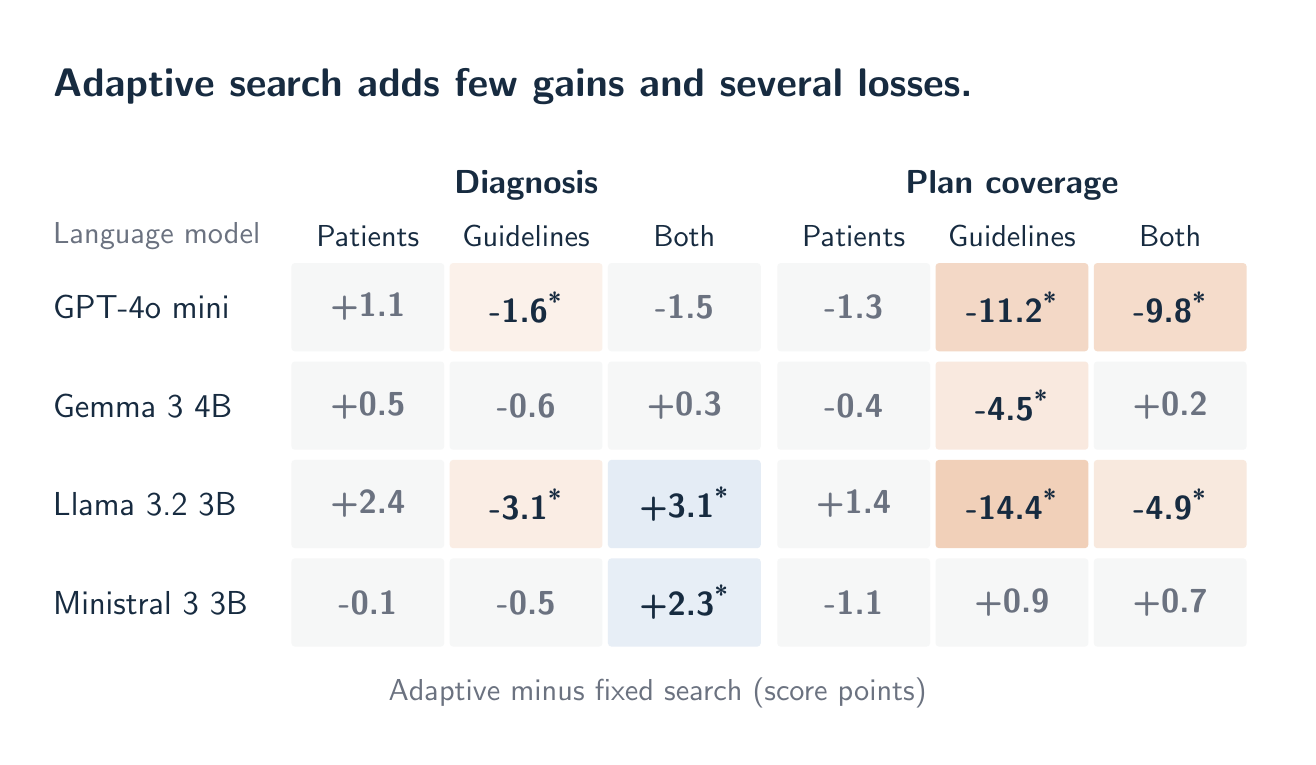
\begin{tikzpicture}[x=1cm,y=1cm]
\definecolor{matrixink}{HTML}{172B40}
\definecolor{matrixmuted}{HTML}{6B7280}
\definecolor{matrixpositive}{HTML}{3E79B8}
\definecolor{matrixnegative}{HTML}{D98042}
\useasboundingbox (0,0) rectangle (16,9);
\fill[white] (0,0) rectangle (16,9);
\node[anchor=west,text=matrixink,font=\fontsize{15}{18}\selectfont\bfseries] at (0.2,8.25) {Adaptive search adds few gains and several losses.};
\node[anchor=west,text=matrixmuted,font=\fontsize{10.5}{12}\selectfont] at (0.2,6.36) {Language model};
\node[text=matrixink,font=\fontsize{12}{14}\selectfont\bfseries] at (6.330,7.0) {Diagnosis};
\node[text=matrixink,font=\fontsize{10.5}{12}\selectfont] at (4.320,6.36) {Patients};
\node[text=matrixink,font=\fontsize{10.5}{12}\selectfont] at (6.330,6.36) {Guidelines};
\node[text=matrixink,font=\fontsize{10.5}{12}\selectfont] at (8.340,6.36) {Both};
\node[text=matrixink,font=\fontsize{12}{14}\selectfont\bfseries] at (12.500,7.0) {Plan coverage};
\node[text=matrixink,font=\fontsize{10.5}{12}\selectfont] at (10.490,6.36) {Patients};
\node[text=matrixink,font=\fontsize{10.5}{12}\selectfont] at (12.500,6.36) {Guidelines};
\node[text=matrixink,font=\fontsize{10.5}{12}\selectfont] at (14.510,6.36) {Both};
\node[anchor=west,text=matrixink,font=\fontsize{11.5}{14}\selectfont] at (0.2,5.450) {GPT-4o mini};
% cell model=gpt_4o_mini metric=diagnosis source=patient_retrieval baseline_variant=patient_retrieval comparison_variant=agentic_patient_retrieval n_pairs=2378 n_patients=2047 mean_baseline=0.8086805609827662 mean_comparison=0.8201086472871351 mean_difference=0.0114280863043687 p_value_two_sided=0.0027974806703352 p_value_two_sided_holm=0.041962210055028 display_value=+1.1 display_significant=False
\fill[matrixink!4,rounded corners=1.2pt] (3.350,4.890) rectangle (5.290,6.010);
\node[text=matrixmuted,font=\fontsize{13}{15}\selectfont\bfseries] at (4.320,5.450) {+1.1};
% cell model=gpt_4o_mini metric=diagnosis source=guidelines baseline_variant=guidelines comparison_variant=agentic_guidelines n_pairs=2370 n_patients=2039 mean_baseline=0.7490407758735221 mean_comparison=0.7335126180402953 mean_difference=-0.0155281578332268 p_value_two_sided=6.228581199501367e-05 p_value_two_sided_holm=0.0012457162399002 display_value=-1.6 display_significant=True
\fill[matrixnegative!11.11,rounded corners=1.2pt] (5.360,4.890) rectangle (7.300,6.010);
\node[text=matrixink,font=\fontsize{13}{15}\selectfont\bfseries] at (6.330,5.450) {-1.6\textsuperscript{*}};
% cell model=gpt_4o_mini metric=diagnosis source=both baseline_variant=patient_retrieval_guidelines comparison_variant=agentic_both n_pairs=2252 n_patients=1955 mean_baseline=0.7839354141214044 mean_comparison=0.7689089391216476 mean_difference=-0.0150264749997567 p_value_two_sided=0.0010971071725187 p_value_two_sided_holm=0.0197479291053379 display_value=-1.5 display_significant=False
\fill[matrixink!4,rounded corners=1.2pt] (7.370,4.890) rectangle (9.310,6.010);
\node[text=matrixmuted,font=\fontsize{13}{15}\selectfont\bfseries] at (8.340,5.450) {-1.5};
% cell model=gpt_4o_mini metric=plan source=patient_retrieval baseline_variant=patient_retrieval comparison_variant=agentic_patient_retrieval n_pairs=2279 n_patients=1976 mean_baseline=0.374981717127395 mean_comparison=0.3624031007751938 mean_difference=-0.0125786163522012 p_value_two_sided=0.1529413264335145 p_value_two_sided_holm=1.0 display_value=-1.3 display_significant=False
\fill[matrixink!4,rounded corners=1.2pt] (9.520,4.890) rectangle (11.460,6.010);
\node[text=matrixmuted,font=\fontsize{13}{15}\selectfont\bfseries] at (10.490,5.450) {-1.3};
% cell model=gpt_4o_mini metric=plan source=guidelines baseline_variant=guidelines comparison_variant=agentic_guidelines n_pairs=2260 n_patients=1957 mean_baseline=0.4056047197640118 mean_comparison=0.2937684365781711 mean_difference=-0.1118362831858407 p_value_two_sided=2.527119709425298e-42 p_value_two_sided_holm=1.036119080864372e-40 display_value=-11.2 display_significant=True
\fill[matrixnegative!30.37,rounded corners=1.2pt] (11.530,4.890) rectangle (13.470,6.010);
\node[text=matrixink,font=\fontsize{13}{15}\selectfont\bfseries] at (12.500,5.450) {-11.2\textsuperscript{*}};
% cell model=gpt_4o_mini metric=plan source=both baseline_variant=patient_retrieval_guidelines comparison_variant=agentic_both n_pairs=2153 n_patients=1886 mean_baseline=0.4337745781080662 mean_comparison=0.3362362594828921 mean_difference=-0.0975383186251741 p_value_two_sided=3.292482204539578e-26 p_value_two_sided_holm=1.1194439495434564e-24 display_value=-9.8 display_significant=True
\fill[matrixnegative!27.51,rounded corners=1.2pt] (13.540,4.890) rectangle (15.480,6.010);
\node[text=matrixink,font=\fontsize{13}{15}\selectfont\bfseries] at (14.510,5.450) {-9.8\textsuperscript{*}};
\node[anchor=west,text=matrixink,font=\fontsize{11.5}{14}\selectfont] at (0.2,4.200) {Gemma 3 4B};
% cell model=ollama_gemma3_4b metric=diagnosis source=patient_retrieval baseline_variant=patient_retrieval comparison_variant=agentic_patient_retrieval n_pairs=2376 n_patients=2046 mean_baseline=0.5013086281331316 mean_comparison=0.5058407808787353 mean_difference=0.0045321527456036 p_value_two_sided=0.4441005312405785 p_value_two_sided_holm=1.0 display_value=+0.5 display_significant=False
\fill[matrixink!4,rounded corners=1.2pt] (3.350,3.640) rectangle (5.290,4.760);
\node[text=matrixmuted,font=\fontsize{13}{15}\selectfont\bfseries] at (4.320,4.200) {+0.5};
% cell model=ollama_gemma3_4b metric=diagnosis source=guidelines baseline_variant=guidelines comparison_variant=agentic_guidelines n_pairs=2370 n_patients=2039 mean_baseline=0.693684404717176 mean_comparison=0.6877352472802052 mean_difference=-0.0059491574369707 p_value_two_sided=0.2629336904451968 p_value_two_sided_holm=1.0 display_value=-0.6 display_significant=False
\fill[matrixink!4,rounded corners=1.2pt] (5.360,3.640) rectangle (7.300,4.760);
\node[text=matrixmuted,font=\fontsize{13}{15}\selectfont\bfseries] at (6.330,4.200) {-0.6};
% cell model=ollama_gemma3_4b metric=diagnosis source=both baseline_variant=patient_retrieval_guidelines comparison_variant=agentic_both n_pairs=2252 n_patients=1955 mean_baseline=0.6784898380241243 mean_comparison=0.6817154213932233 mean_difference=0.0032255833690989 p_value_two_sided=0.6107498824558152 p_value_two_sided_holm=1.0 display_value=+0.3 display_significant=False
\fill[matrixink!4,rounded corners=1.2pt] (7.370,3.640) rectangle (9.310,4.760);
\node[text=matrixmuted,font=\fontsize{13}{15}\selectfont\bfseries] at (8.340,4.200) {+0.3};
% cell model=ollama_gemma3_4b metric=plan source=patient_retrieval baseline_variant=patient_retrieval comparison_variant=agentic_patient_retrieval n_pairs=2270 n_patients=1967 mean_baseline=0.1564977973568282 mean_comparison=0.1520558002936857 mean_difference=-0.0044419970631424 p_value_two_sided=0.4517024878703083 p_value_two_sided_holm=1.0 display_value=-0.4 display_significant=False
\fill[matrixink!4,rounded corners=1.2pt] (9.520,3.640) rectangle (11.460,4.760);
\node[text=matrixmuted,font=\fontsize{13}{15}\selectfont\bfseries] at (10.490,4.200) {-0.4};
% cell model=ollama_gemma3_4b metric=plan source=guidelines baseline_variant=guidelines comparison_variant=agentic_guidelines n_pairs=2240 n_patients=1943 mean_baseline=0.2854166666666666 mean_comparison=0.2399553571428571 mean_difference=-0.0454613095238095 p_value_two_sided=4.063597801088753e-08 p_value_two_sided_holm=1.0971714062939633e-06 display_value=-4.5 display_significant=True
\fill[matrixnegative!17.09,rounded corners=1.2pt] (11.530,3.640) rectangle (13.470,4.760);
\node[text=matrixink,font=\fontsize{13}{15}\selectfont\bfseries] at (12.500,4.200) {-4.5\textsuperscript{*}};
% cell model=ollama_gemma3_4b metric=plan source=both baseline_variant=patient_retrieval_guidelines comparison_variant=agentic_both n_pairs=2156 n_patients=1886 mean_baseline=0.245091218305504 mean_comparison=0.2466759431045145 mean_difference=0.0015847247990105 p_value_two_sided=0.8428869417924316 p_value_two_sided_holm=1.0 display_value=+0.2 display_significant=False
\fill[matrixink!4,rounded corners=1.2pt] (13.540,3.640) rectangle (15.480,4.760);
\node[text=matrixmuted,font=\fontsize{13}{15}\selectfont\bfseries] at (14.510,4.200) {+0.2};
\node[anchor=west,text=matrixink,font=\fontsize{11.5}{14}\selectfont] at (0.2,2.950) {Llama 3.2 3B};
% cell model=ollama_llama3_2_3b metric=diagnosis source=patient_retrieval baseline_variant=patient_retrieval comparison_variant=agentic_patient_retrieval n_pairs=2378 n_patients=2047 mean_baseline=0.508836536416325 mean_comparison=0.5329961687089223 mean_difference=0.0241596322925972 p_value_two_sided=0.0012310868268135 p_value_two_sided_holm=0.0209284760558302 display_value=+2.4 display_significant=False
\fill[matrixink!4,rounded corners=1.2pt] (3.350,2.390) rectangle (5.290,3.510);
\node[text=matrixmuted,font=\fontsize{13}{15}\selectfont\bfseries] at (4.320,2.950) {+2.4};
% cell model=ollama_llama3_2_3b metric=diagnosis source=guidelines baseline_variant=guidelines comparison_variant=agentic_guidelines n_pairs=2370 n_patients=2039 mean_baseline=0.6646884346145342 mean_comparison=0.6341004946819564 mean_difference=-0.0305879399325776 p_value_two_sided=6.199272104682623e-08 p_value_two_sided_holm=1.611810747217482e-06 display_value=-3.1 display_significant=True
\fill[matrixnegative!14.12,rounded corners=1.2pt] (5.360,2.390) rectangle (7.300,3.510);
\node[text=matrixink,font=\fontsize{13}{15}\selectfont\bfseries] at (6.330,2.950) {-3.1\textsuperscript{*}};
% cell model=ollama_llama3_2_3b metric=diagnosis source=both baseline_variant=patient_retrieval_guidelines comparison_variant=agentic_both n_pairs=2252 n_patients=1955 mean_baseline=0.5918840471582564 mean_comparison=0.6224947850190556 mean_difference=0.0306107378607991 p_value_two_sided=3.5294585823565274e-05 p_value_two_sided_holm=0.0007411863022948 display_value=+3.1 display_significant=True
\fill[matrixpositive!14.12,rounded corners=1.2pt] (7.370,2.390) rectangle (9.310,3.510);
\node[text=matrixink,font=\fontsize{13}{15}\selectfont\bfseries] at (8.340,2.950) {+3.1\textsuperscript{*}};
% cell model=ollama_llama3_2_3b metric=plan source=patient_retrieval baseline_variant=patient_retrieval comparison_variant=agentic_patient_retrieval n_pairs=2298 n_patients=1989 mean_baseline=0.1961125616478096 mean_comparison=0.2097476066144473 mean_difference=0.0136350449666376 p_value_two_sided=0.1063458446849359 p_value_two_sided_holm=1.0 display_value=+1.4 display_significant=False
\fill[matrixink!4,rounded corners=1.2pt] (9.520,2.390) rectangle (11.460,3.510);
\node[text=matrixmuted,font=\fontsize{13}{15}\selectfont\bfseries] at (10.490,2.950) {+1.4};
% cell model=ollama_llama3_2_3b metric=plan source=guidelines baseline_variant=guidelines comparison_variant=agentic_guidelines n_pairs=2283 n_patients=1977 mean_baseline=0.337275514673675 mean_comparison=0.1929478756022777 mean_difference=-0.1443276390713972 p_value_two_sided=6.026684759118117e-71 p_value_two_sided_holm=2.7120081416031523e-69 display_value=-14.4 display_significant=True
\fill[matrixnegative!36.87,rounded corners=1.2pt] (11.530,2.390) rectangle (13.470,3.510);
\node[text=matrixink,font=\fontsize{13}{15}\selectfont\bfseries] at (12.500,2.950) {-14.4\textsuperscript{*}};
% cell model=ollama_llama3_2_3b metric=plan source=both baseline_variant=patient_retrieval_guidelines comparison_variant=agentic_both n_pairs=2167 n_patients=1895 mean_baseline=0.2979157052761113 mean_comparison=0.2493462544223965 mean_difference=-0.0485694508537148 p_value_two_sided=4.386405098074493e-07 p_value_two_sided_holm=1.0527372235378784e-05 display_value=-4.9 display_significant=True
\fill[matrixnegative!17.71,rounded corners=1.2pt] (13.540,2.390) rectangle (15.480,3.510);
\node[text=matrixink,font=\fontsize{13}{15}\selectfont\bfseries] at (14.510,2.950) {-4.9\textsuperscript{*}};
\node[anchor=west,text=matrixink,font=\fontsize{11.5}{14}\selectfont] at (0.2,1.700) {Ministral 3 3B};
% cell model=ollama_ministral_3_3b metric=diagnosis source=patient_retrieval baseline_variant=patient_retrieval comparison_variant=agentic_patient_retrieval n_pairs=2378 n_patients=2047 mean_baseline=0.5649872585216635 mean_comparison=0.5639797175263126 mean_difference=-0.0010075409953508 p_value_two_sided=0.8678543643851234 p_value_two_sided_holm=1.0 display_value=-0.1 display_significant=False
\fill[matrixink!4,rounded corners=1.2pt] (3.350,1.140) rectangle (5.290,2.260);
\node[text=matrixmuted,font=\fontsize{13}{15}\selectfont\bfseries] at (4.320,1.700) {-0.1};
% cell model=ollama_ministral_3_3b metric=diagnosis source=guidelines baseline_variant=guidelines comparison_variant=agentic_guidelines n_pairs=2370 n_patients=2039 mean_baseline=0.604220323331487 mean_comparison=0.5993158542636501 mean_difference=-0.0049044690678369 p_value_two_sided=0.3905732349145149 p_value_two_sided_holm=1.0 display_value=-0.5 display_significant=False
\fill[matrixink!4,rounded corners=1.2pt] (5.360,1.140) rectangle (7.300,2.260);
\node[text=matrixmuted,font=\fontsize{13}{15}\selectfont\bfseries] at (6.330,1.700) {-0.5};
% cell model=ollama_ministral_3_3b metric=diagnosis source=both baseline_variant=patient_retrieval_guidelines comparison_variant=agentic_both n_pairs=2252 n_patients=1955 mean_baseline=0.6013641573554546 mean_comparison=0.6240423640274358 mean_difference=0.0226782066719812 p_value_two_sided=0.0001484845432137 p_value_two_sided_holm=0.0028212063210617 display_value=+2.3 display_significant=True
\fill[matrixpositive!12.54,rounded corners=1.2pt] (7.370,1.140) rectangle (9.310,2.260);
\node[text=matrixink,font=\fontsize{13}{15}\selectfont\bfseries] at (8.340,1.700) {+2.3\textsuperscript{*}};
% cell model=ollama_ministral_3_3b metric=plan source=patient_retrieval baseline_variant=patient_retrieval comparison_variant=agentic_patient_retrieval n_pairs=2302 n_patients=1994 mean_baseline=0.3249710396756443 mean_comparison=0.3143643208803938 mean_difference=-0.0106067187952505 p_value_two_sided=0.1800959504409327 p_value_two_sided_holm=1.0 display_value=-1.1 display_significant=False
\fill[matrixink!4,rounded corners=1.2pt] (9.520,1.140) rectangle (11.460,2.260);
\node[text=matrixmuted,font=\fontsize{13}{15}\selectfont\bfseries] at (10.490,1.700) {-1.1};
% cell model=ollama_ministral_3_3b metric=plan source=guidelines baseline_variant=guidelines comparison_variant=agentic_guidelines n_pairs=2285 n_patients=1977 mean_baseline=0.3838803792851932 mean_comparison=0.3927425237053246 mean_difference=0.0088621444201312 p_value_two_sided=0.290873870055003 p_value_two_sided_holm=1.0 display_value=+0.9 display_significant=False
\fill[matrixink!4,rounded corners=1.2pt] (11.530,1.140) rectangle (13.470,2.260);
\node[text=matrixmuted,font=\fontsize{13}{15}\selectfont\bfseries] at (12.500,1.700) {+0.9};
% cell model=ollama_ministral_3_3b metric=plan source=both baseline_variant=patient_retrieval_guidelines comparison_variant=agentic_both n_pairs=2171 n_patients=1900 mean_baseline=0.3798172884999232 mean_comparison=0.3868800859818824 mean_difference=0.0070627974819591 p_value_two_sided=0.4162649201313345 p_value_two_sided_holm=1.0 display_value=+0.7 display_significant=False
\fill[matrixink!4,rounded corners=1.2pt] (13.540,1.140) rectangle (15.480,2.260);
\node[text=matrixmuted,font=\fontsize{13}{15}\selectfont\bfseries] at (14.510,1.700) {+0.7};
\node[text=matrixmuted,font=\fontsize{10.5}{12}\selectfont] at (8,0.55) {Adaptive minus fixed search (score points)};
\end{tikzpicture}
\par\centering\vspace{1mm}
{\fontsize{8}{10}\selectfont\color{black!65}* Holm-adjusted $p<.01$ (48 comparisons).\par}
\end{minipage}
\end{document}
